\documentclass[12pt,a4paper]{article}

% ── Packages ──────────────────────────────────────────────
\usepackage[a4paper, top=1in, bottom=1in, left=1.1in, right=1.1in, headheight=15pt]{geometry}
\usepackage[T1]{fontenc}
\usepackage[utf8]{inputenc}
\usepackage{graphicx}
\usepackage{amsmath}
\usepackage{booktabs}
\usepackage{longtable}
\usepackage{array}
\usepackage{xcolor}
\usepackage{colortbl}
\usepackage{hyperref}
\usepackage{enumitem}
\usepackage{titlesec}
\usepackage{fancyhdr}
\usepackage{tikz}
\usepackage{multirow}
\usepackage{tabularx}
\usepackage{setspace}
\usepackage{mdframed}
\usepackage{listings}
\usepackage{caption}
\usepackage{float}
\usepackage{pgfplots}
\pgfplotsset{compat=1.18}
\usetikzlibrary{shapes.geometric, arrows.meta, positioning, fit, backgrounds,
                mindmap, trees, shadows, decorations.pathmorphing, calc}

% ── Colors ────────────────────────────────────────────────
\definecolor{primaryblue}{RGB}{30, 100, 180}
\definecolor{accentorange}{RGB}{220, 80, 30}
\definecolor{lightgray}{RGB}{245, 245, 245}
\definecolor{darkgray}{RGB}{60, 60, 60}
\definecolor{successgreen}{RGB}{34, 139, 34}
\definecolor{warningred}{RGB}{180, 30, 30}
\definecolor{sectionblue}{RGB}{20, 80, 160}
\definecolor{tablebg}{RGB}{248, 250, 255}

% ── Hyperref setup ─────────────────────────────────────────
\hypersetup{
    colorlinks=true,
    linkcolor=primaryblue,
    urlcolor=primaryblue,
    citecolor=primaryblue,
    pdftitle={Bihar Sahayata - Project Synopsis},
    pdfauthor={Shubham Kumar Mishra, Atul Sharma}
}

% ── Section formatting ─────────────────────────────────────
\titleformat{\section}
  {\large\bfseries\color{sectionblue}}
  {\thesection.}{0.6em}{}
  [\vspace{-0.3em}\textcolor{sectionblue}{\rule{\linewidth}{0.6pt}}]

\titleformat{\subsection}
  {\normalsize\bfseries\color{darkgray}}
  {\thesubsection.}{0.5em}{}

\titlespacing{\section}{0pt}{14pt}{8pt}
\titlespacing{\subsection}{0pt}{10pt}{5pt}

% ── Header / Footer ───────────────────────────────────────
\pagestyle{fancy}
\fancyhf{}
\fancyhead[L]{\small\textcolor{primaryblue}{\textbf{Bihar Sahayata}}}
\fancyhead[R]{\small\textcolor{darkgray}{BCA Project Synopsis --- Patna University}}
\fancyfoot[C]{\small\thepage}
\renewcommand{\headrulewidth}{0.4pt}
\renewcommand{\footrulewidth}{0.4pt}

% ── Table helper ──────────────────────────────────────────
\newcolumntype{L}[1]{>{\raggedright\arraybackslash}p{#1}}
\newcolumntype{C}[1]{>{\centering\arraybackslash}p{#1}}
\newcolumntype{R}[1]{>{\raggedleft\arraybackslash}p{#1}}

% ── TikZ node styles ─────────────────────────────────────
\tikzset{
  box/.style={rectangle, rounded corners=4pt, draw=primaryblue,
              fill=primaryblue!8, text width=#1, align=center,
              minimum height=1cm, font=\small, inner sep=4pt},
  box/.default=3cm,
  adminbox/.style={rectangle, rounded corners=4pt, draw=warningred,
              fill=warningred!8, text width=#1, align=center,
              minimum height=1cm, font=\small, inner sep=4pt},
  adminbox/.default=2.8cm,
  volbox/.style={rectangle, rounded corners=4pt, draw=successgreen,
              fill=successgreen!8, text width=#1, align=center,
              minimum height=1cm, font=\small, inner sep=4pt},
  volbox/.default=2.8cm,
  dbbox/.style={cylinder, shape border rotate=90, draw=darkgray,
              fill=lightgray, text width=2.4cm, align=center,
              minimum height=1.4cm, font=\small},
  cloudbox/.style={rectangle, rounded corners=8pt, draw=accentorange,
              fill=accentorange!8, text width=#1, align=center,
              minimum height=1cm, font=\small, inner sep=4pt},
  cloudbox/.default=2.8cm,
  arrow/.style={-{Stealth[scale=1.1]}, thick, color=darkgray},
  dasharrow/.style={-{Stealth[scale=1.1]}, dashed, thick, color=darkgray!60},
}

\begin{document}

% ═══════════════════════════════════════════════════════════
%  TITLE PAGE
% ═══════════════════════════════════════════════════════════
\begin{titlepage}
\centering
\vspace*{0.6cm}

{\Large\bfseries\color{primaryblue} PATNA UNIVERSITY}\\[0.3cm]
{\normalsize Department of Computer Applications}\\[0.1cm]
{\normalsize Bachelor of Computer Applications (BCA) --- Semester V}\\[1cm]

\noindent\textcolor{primaryblue}{\rule{\textwidth}{1.5pt}}\\[0.5cm]

{\Huge\bfseries\color{accentorange} PROJECT SYNOPSIS}\\[0.4cm]

\noindent\textcolor{primaryblue}{\rule{\textwidth}{1.5pt}}\\[1.4cm]

\begin{mdframed}[linecolor=primaryblue, linewidth=2pt,
                  innertopmargin=14pt, innerbottommargin=14pt,
                  backgroundcolor=primaryblue!5]
\centering
{\LARGE\bfseries\color{primaryblue} Bihar Sahayata}\\[0.4cm]
{\large\color{darkgray} A Disaster Relief \& Emergency Coordination Platform}\\[0.25cm]
{\normalsize\color{darkgray!80} Real-time volunteer coordination, emergency SOS,
and relief fund management for Bihar}
\end{mdframed}

\vspace{1.6cm}

\begin{tabular}{@{}L{5.5cm} @{}c@{\hspace{4pt}} L{8cm}}
\textbf{Student Names}   & : & Shubham Kumar Mishra \& Atul Sharma \\[0.5cm]
\textbf{Roll Numbers}    & : & 23\ \ (Shubham Kumar Mishra) \\
                         &   & 10\ \ (Atul Sharma) \\[0.5cm]
\textbf{Course}          & : & BCA --- Semester V \\[0.5cm]
\textbf{Batch / Session} & : & 2023--2026 \\[0.5cm]
\textbf{Project Guide}   & : & \underline{\hspace{6.5cm}} \\[0.5cm]
\textbf{Designation}     & : & \underline{\hspace{6.5cm}} \\[0.5cm]
\textbf{College Name}    & : & \underline{\hspace{6.5cm}} \\[0.5cm]
\end{tabular}

\vfill

\begin{tabular}{@{}L{5cm} L{5cm} L{4cm}}
\textbf{Student Signature} & \textbf{Guide Signature} & \textbf{HOD Signature} \\[1.4cm]
\underline{\hspace{4cm}} & \underline{\hspace{4cm}} & \underline{\hspace{3cm}} \\
\end{tabular}

\vspace{1cm}
{\small Session: 2025--2026}
\end{titlepage}

% ═══════════════════════════════════════════════════════════
\setcounter{page}{1}
\onehalfspacing

% ═══════════════════════════════════════════════════════════
%  1. INTRODUCTION
% ═══════════════════════════════════════════════════════════
\section{Introduction}

Bihar is one of the most disaster-prone states in India, experiencing
annual floods caused by the rivers Ganga, Kosi, Gandak, and Bagmati.
According to the National Disaster Management Authority (NDMA), nearly
73\% of Bihar's geographical area is flood-affected, displacing millions
of people every year. Despite having a large volunteer base and active
NGOs, the coordination between citizens in distress, volunteers, and
disaster management authorities remains fragmented, slow, and largely
paper-based.

\textbf{Bihar Sahayata} is a full-stack, mobile-first disaster relief and
emergency coordination platform designed specifically for the state of Bihar.
The platform addresses the critical gap between citizens who need help and
the volunteers and authorities who can provide it --- enabling real-time
emergency reporting, volunteer dispatch, team coordination, and transparent
relief fund management on a single unified system.

The project provides three distinct interfaces for three distinct roles:

\begin{enumerate}[leftmargin=*, label=\textbf{\arabic*.}, itemsep=3pt]
  \item \textbf{Citizens} can send SOS panic alerts with GPS location,
        report issues such as flooding, medical emergencies, or infrastructure
        damage, and donate to verified relief campaigns.
  \item \textbf{Volunteers} can receive nearby alerts, accept and resolve
        issues, join or form rescue teams, and track their service history.
  \item \textbf{Administrators / Authorities} can declare official disasters,
        activate volunteer teams, monitor all active issues across districts,
        approve fundraising campaigns, and dispatch bulk notifications.
\end{enumerate}

The system is built to work on low-bandwidth mobile connections using a
React Native mobile application backed by a production-grade Node.js REST API,
ensuring accessibility even in disaster-affected areas with limited connectivity.

% ═══════════════════════════════════════════════════════════
%  2. OBJECTIVES
% ═══════════════════════════════════════════════════════════
\section{Objectives of the Project}

\begin{enumerate}[leftmargin=*, label=\textbf{\arabic*.}, itemsep=4pt]
  \item \textbf{Emergency SOS System:} Provide a one-tap panic alert mechanism
        that captures the citizen's GPS coordinates and instantly identifies nearby
        verified volunteers within a 20\,km radius.

  \item \textbf{Issue Reporting and Tracking:} Enable citizens to report structured
        emergency issues (flood, medical, rescue, etc.) with severity levels, victim
        details, and location --- and track the status of their reports from
        \textit{pending} through to \textit{resolved}.

  \item \textbf{Volunteer Coordination:} Build a volunteer management system that
        allows verified volunteers to accept, respond to, and resolve issues through
        a defined workflow: Accepted $\rightarrow$ En Route $\rightarrow$ On Site
        $\rightarrow$ Resolved.

  \item \textbf{Team Management:} Allow volunteers to form rescue, medical, relief,
        or general teams, manage membership, and be activated by administrators
        during declared disasters.

  \item \textbf{Disaster Management Dashboard:} Provide administrators with tools
        to declare official disasters, monitor affected districts, activate volunteer
        teams, and update disaster status in real time.

  \item \textbf{Transparent Crowdfunding:} Enable creation of verified relief
        campaigns with goal amounts, donor tracking, and progress transparency ---
        so the public can donate with confidence.

  \item \textbf{Role-Based Access Control:} Enforce strict separation of
        permissions between citizens (\texttt{user}), field workers
        (\texttt{volunteer}), and authorities (\texttt{admin}).

  \item \textbf{Cross-Platform Accessibility:} Deliver the platform as a
        React Native mobile application accessible on both Android and iOS,
        with a shared backend serving both mobile and web clients.
\end{enumerate}

% ═══════════════════════════════════════════════════════════
%  3. SCOPE
% ═══════════════════════════════════════════════════════════
\section{Scope of the Project}

\subsection{In Scope}

\begin{itemize}[leftmargin=*, itemsep=3pt]
  \item Emergency SOS alerts with geolocation and countdown timer.
  \item Multi-step issue reporting with severity, victim details, and GPS.
  \item Full volunteer lifecycle: onboarding, verification, qualification
        tracking, team membership, and issue resolution.
  \item Disaster declaration, team activation, and status management by
        administrators.
  \item Campaign creation, admin approval workflow, and donation processing
        (demo payment gateway included; production Razorpay-ready).
  \item Role-based dashboards for users, volunteers, and admins.
  \item All 38 Bihar districts seeded and searchable.
  \item REST API deployed on cloud infrastructure (Fly.io) with Docker.
  \item Email verification and password reset via Resend email service.
  \item Google OAuth social login in addition to email/password.
  \item OpenAPI documentation for all endpoints.
\end{itemize}

\subsection{Out of Scope (Future Enhancements)}

\begin{itemize}[leftmargin=*, itemsep=3pt]
  \item Live real-time push notifications (Firebase Cloud Messaging --- planned).
  \item WebSocket-based real-time status updates.
  \item SMS alerts for non-smartphone users (MSG91 / Twilio --- planned).
  \item Live volunteer location tracking on map.
  \item AI-based severity prediction and volunteer auto-assignment.
  \item Integration with government SDMA (State Disaster Management Authority) APIs.
\end{itemize}

% ═══════════════════════════════════════════════════════════
%  4. METHODOLOGY
% ═══════════════════════════════════════════════════════════
\section{Methodology}

The project follows the \textbf{Agile Software Development} methodology,
with development divided into eight focused phases, each producing a
working, testable increment.

\subsection{Development Phases}

\vspace{0.4cm}
\begin{center}
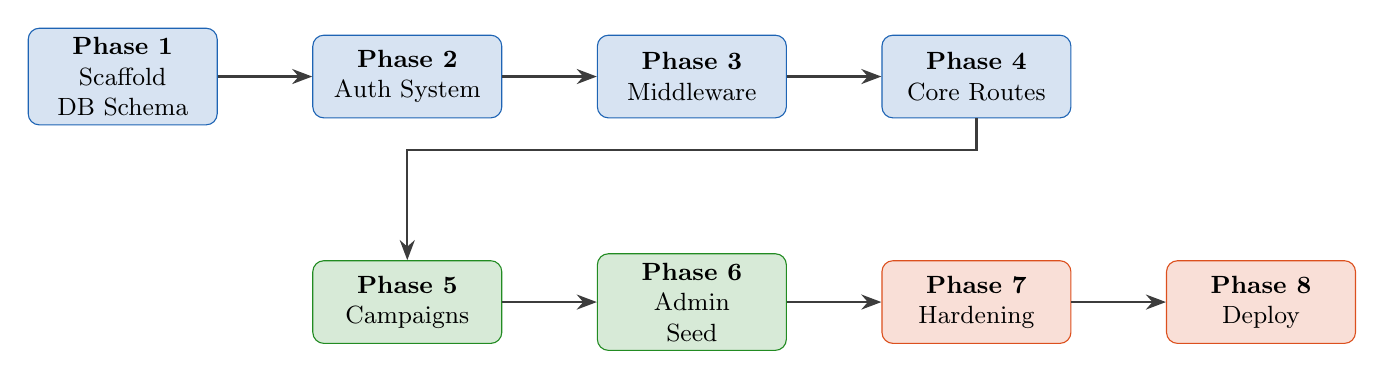
\begin{tikzpicture}[node distance=1.5cm and 1.2cm, every node/.style={font=\small, align=center}, transform shape]
  \node[rectangle, draw=primaryblue, rounded corners=4pt, fill=primaryblue!18, minimum width=2.4cm, minimum height=1.05cm] (p1)
        {\textbf{Phase 1}\\Scaffold \\DB Schema};
  \node[rectangle, draw=primaryblue, rounded corners=4pt, fill=primaryblue!18, right=1.2cm of p1, minimum width=2.4cm, minimum height=1.05cm] (p2)
        {\textbf{Phase 2}\\Auth System};
  \node[rectangle, draw=primaryblue, rounded corners=4pt, fill=primaryblue!18, right=1.2cm of p2, minimum width=2.4cm, minimum height=1.05cm] (p3)
        {\textbf{Phase 3}\\Middleware};
  \node[rectangle, draw=primaryblue, rounded corners=4pt, fill=primaryblue!18, right=1.2cm of p3, minimum width=2.4cm, minimum height=1.05cm] (p4)
        {\textbf{Phase 4}\\Core Routes};

  \node[rectangle, draw=successgreen, rounded corners=4pt, fill=successgreen!18, below=1.8cm of p2, minimum width=2.4cm, minimum height=1.05cm] (p5)
        {\textbf{Phase 5}\\Campaigns};
  \node[rectangle, draw=successgreen, rounded corners=4pt, fill=successgreen!18, right=1.2cm of p5, minimum width=2.4cm, minimum height=1.05cm] (p6)
        {\textbf{Phase 6}\\Admin \\Seed};
  \node[rectangle, draw=accentorange, rounded corners=4pt, fill=accentorange!18, right=1.2cm of p6, minimum width=2.4cm, minimum height=1.05cm] (p7)
        {\textbf{Phase 7}\\Hardening};
  \node[rectangle, draw=accentorange, rounded corners=4pt, fill=accentorange!18, right=1.2cm of p7, minimum width=2.4cm, minimum height=1.05cm] (p8)
        {\textbf{Phase 8}\\Deploy};

  \draw[arrow] (p1) -- (p2);
  \draw[arrow] (p2) -- (p3);
  \draw[arrow] (p3) -- (p4);
  \draw[arrow] (p4.south) -- ++(0,-0.4) -| (p5.north);
  \draw[arrow] (p5) -- (p6);
  \draw[arrow] (p6) -- (p7);
  \draw[arrow] (p7) -- (p8);
\end{tikzpicture}
\end{center}
\vspace{0.3cm}

\newpage
\subsection{Issue Resolution Workflow}

The core workflow follows a simple state progression with an escalation path:

\vspace{0.4cm}
\begin{center}
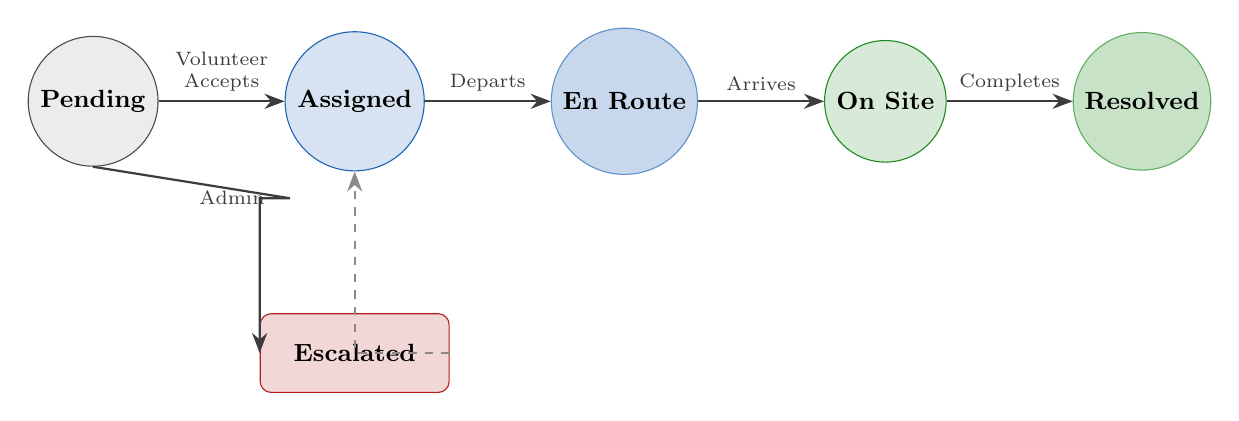
\begin{tikzpicture}[node distance=1.7cm and 1.4cm, every node/.style={font=\small, align=center}, transform shape]
  \node[circle, draw=black!70, fill=gray!15, minimum size=1.2cm] (pending)
        {\textbf{Pending}};
  \node[circle, draw=primaryblue, fill=primaryblue!18, right=1.6cm of pending, minimum size=1.2cm] (assigned)
        {\textbf{Assigned}};
  \node[circle, draw=primaryblue!70, fill=primaryblue!25, right=1.6cm of assigned, minimum size=1.2cm] (enroute)
        {\textbf{En Route}};
  \node[circle, draw=successgreen, fill=successgreen!18, right=1.6cm of enroute, minimum size=1.2cm] (onsite)
        {\textbf{On Site}};
  \node[circle, draw=successgreen!70, fill=successgreen!25, right=1.6cm of onsite, minimum size=1.2cm] (resolved)
        {\textbf{Resolved}};
  \node[rectangle, draw=warningred, rounded corners=4pt, fill=warningred!18, below=1.8cm of assigned, minimum width=2.4cm, minimum height=1.0cm] (escalated)
        {\textbf{Escalated}};

  \draw[arrow] (pending) -- node[above,font=\scriptsize,align=center]{Volunteer\\Accepts} (assigned);
  \draw[arrow] (assigned) -- node[above,font=\scriptsize]{Departs} (enroute);
  \draw[arrow] (enroute) -- node[above,font=\scriptsize]{Arrives} (onsite);
  \draw[arrow] (onsite) -- node[above,font=\scriptsize]{Completes} (resolved);
  \draw[arrow] (pending.south) -- ++(2.5,-0.4) -| node[near start,left,font=\scriptsize]{Admin} (escalated.west);
  \draw[dasharrow] (escalated.east) -| (assigned.south);
\end{tikzpicture}
\end{center}
\vspace{0.3cm}

\subsection{Volunteer Geolocation Algorithm}

To find nearby volunteers for panic alerts and high-severity issues,
the system uses the \textbf{Haversine Formula} on the PostgreSQL database,
computing great-circle distances between the issue GPS coordinates and
each volunteer's registered location:

\[
d = 2r \cdot \arcsin\!\left(\sqrt{
  \sin^2\!\left(\dfrac{\phi_2 - \phi_1}{2}\right)
  + \cos\phi_1 \cos\phi_2 \sin^2\!\left(\dfrac{\lambda_2 - \lambda_1}{2}\right)
}\right)
\]

where $r = 6371$\,km (Earth's radius), $\phi$ = latitude, $\lambda$ = longitude.
Volunteers within \textbf{20\,km} of a panic alert and \textbf{15\,km}
of a high-severity issue are identified and notified.

\newpage
% ═══════════════════════════════════════════════════════════
%  5. SYSTEM ARCHITECTURE
% ═══════════════════════════════════════════════════════════
\section{System Architecture}

\subsection{High-Level Architecture}

\vspace{0.4cm}
\begin{center}
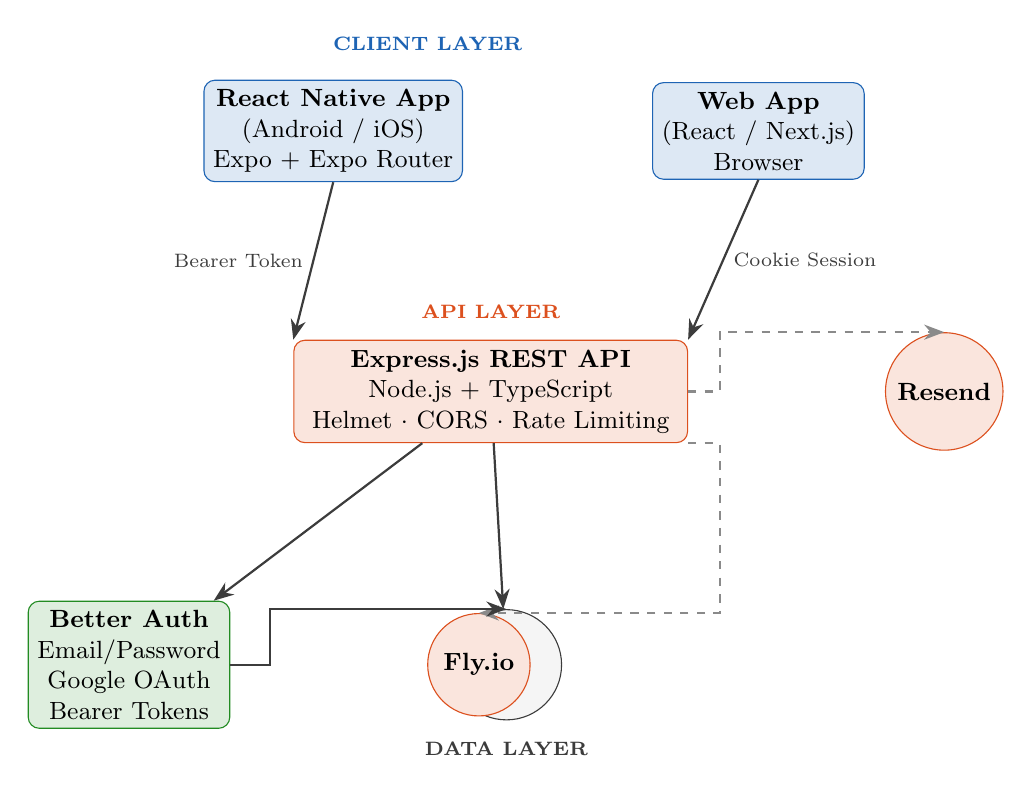
\begin{tikzpicture}[node distance=1.8cm and 1.8cm, every node/.style={font=\small, align=center}, transform shape]
  \node[rectangle, draw=primaryblue, rounded corners=4pt, fill=primaryblue!15, minimum width=2.4cm, minimum height=1.1cm] (rn)
        {\textbf{React Native App}\\(Android / iOS)\\Expo + Expo Router};
  \node[rectangle, draw=primaryblue, rounded corners=4pt, fill=primaryblue!15, minimum width=2.4cm, minimum height=1.1cm, right=2.4cm of rn] (web)
        {\textbf{Web App}\\(React / Next.js)\\Browser};

  \node[rectangle, draw=accentorange, rounded corners=4pt, fill=accentorange!15, minimum width=5cm, minimum height=1.3cm, below=2.0cm of rn, xshift=2.0cm] (api)
        {\textbf{Express.js REST API}\\Node.js + TypeScript\\Helmet $\cdot$ CORS $\cdot$ Rate Limiting};

  \node[rectangle, draw=successgreen, rounded corners=4pt, fill=successgreen!15, minimum width=2.4cm, minimum height=1.05cm, below left=2.0cm and 0.8cm of api] (auth)
        {\textbf{Better Auth}\\Email/Password\\Google OAuth\\Bearer Tokens};
  \node[circle, draw=darkgray, fill=lightgray, minimum size=1.4cm, right=2.8cm of auth] (db)
        {\textbf{DB}};

  \node[circle, draw=accentorange, fill=accentorange!15, minimum size=1.3cm, right=2.5cm of api] (resend)
        {\textbf{Resend}};
  \node[circle, draw=accentorange, fill=accentorange!15, minimum size=1.3cm, right=2.5cm of auth] (fly)
        {\textbf{Fly.io}};

  \draw[arrow] (rn.south) -- node[left,font=\scriptsize]{Bearer Token} (api.north west);
  \draw[arrow] (web.south) -- node[right,font=\scriptsize]{Cookie Session} (api.north east);
  \draw[arrow] (api) -- (auth);
  \draw[arrow] (api) -- (db);
  \draw[dasharrow] (api.east) -- ++(0.4,0) |- (resend.north);
  \draw[dasharrow] (api.south east) -- ++(0.4,0) |- (fly.north);
  \draw[arrow] (auth.east) -- ++(0.5,0) |- (db.north);

  \node[font=\scriptsize\bfseries, color=primaryblue, above=0.25cm of rn, xshift=1.2cm]
       {CLIENT LAYER};
  \node[font=\scriptsize\bfseries, color=accentorange, above=0.15cm of api]
       {API LAYER};
  \node[font=\scriptsize\bfseries, color=darkgray, below=0.15cm of db]
       {DATA LAYER};
\end{tikzpicture}
\end{center}
\vspace{0.4cm}

\subsection{Database Schema Overview}

The database consists of 19 tables across five functional domains:

\vspace{0.4cm}
\begin{center}
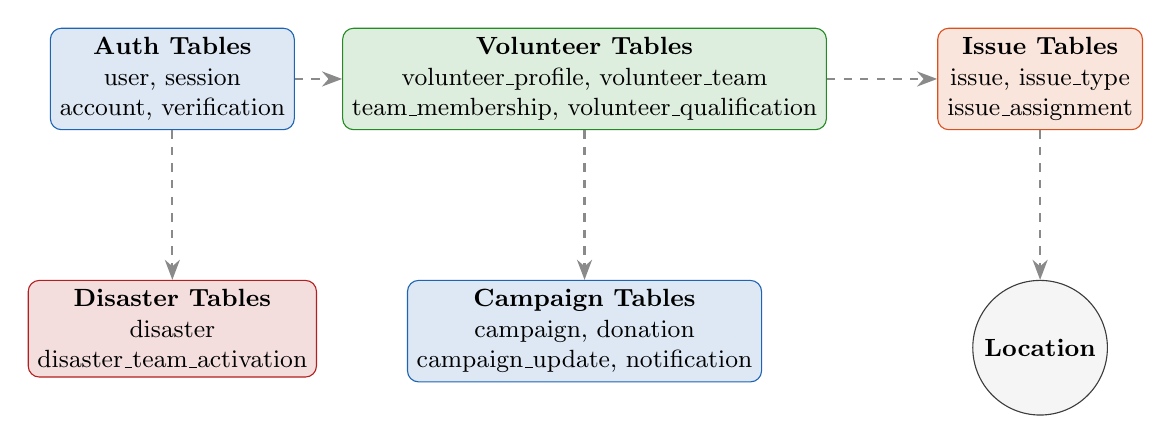
\begin{tikzpicture}[every node/.style={font=\small, align=center}, node distance=1.2cm and 1.4cm, transform shape, xshift=- 1cm]
  \node[rectangle, draw=primaryblue, rounded corners=4pt, fill=primaryblue!15, minimum width=2.0cm, minimum height=1.1cm] (auth_t)
        {\textbf{Auth Tables}\\user, session\\account, verification};
  \node[rectangle, draw=successgreen, rounded corners=4pt, fill=successgreen!15, minimum width=2.6cm, minimum height=1.1cm, right= 0.6cm of auth_t] (vol_t)
        {\textbf{Volunteer Tables}\\volunteer\_profile, volunteer\_team\\team\_membership, volunteer\_qualification};
  \node[rectangle, draw=accentorange, rounded corners=4pt, fill=accentorange!15, minimum width=2.6cm, minimum height=1.1cm, right=1.4cm of vol_t] (issue_t)
        {\textbf{Issue Tables}\\issue, issue\_type\\issue\_assignment};

  \node[rectangle, draw=warningred, rounded corners=4pt, fill=warningred!15, minimum width=2.6cm, minimum height=1.1cm, below=1.9cm of auth_t] (dis_t)
        {\textbf{Disaster Tables}\\disaster\\disaster\_team\_activation};
  \node[rectangle, draw=primaryblue, rounded corners=4pt, fill=primaryblue!15, minimum width=2.6cm, minimum height=1.1cm, below=1.9cm of vol_t] (camp_t)
        {\textbf{Campaign Tables}\\campaign, donation\\campaign\_update, notification};
  \node[circle, draw=darkgray, fill=lightgray, minimum size=1.4cm, below=1.9cm of issue_t] (loc_t)
        {\textbf{Location}};

  \draw[dasharrow] (auth_t.east) -- (vol_t.west);
  \draw[dasharrow] (vol_t.east) -- (issue_t.west);
  \draw[dasharrow] (auth_t.south) -- ++(0,-0.3) -| (dis_t.north);
  \draw[dasharrow] (vol_t.south) -- ++(0,-0.3) -| (camp_t.north);
  \draw[dasharrow] (issue_t.south) -- ++(0,-0.3) -| (loc_t.north);
\end{tikzpicture}
\end{center}
\vspace{0.4cm}

\subsection{Authentication Flow}

Bihar Sahayata uses \textbf{Better Auth} with dual-mode session support,
allowing the same backend to serve both web (cookies) and mobile (bearer tokens):

\vspace{0.4cm}
\begin{center}
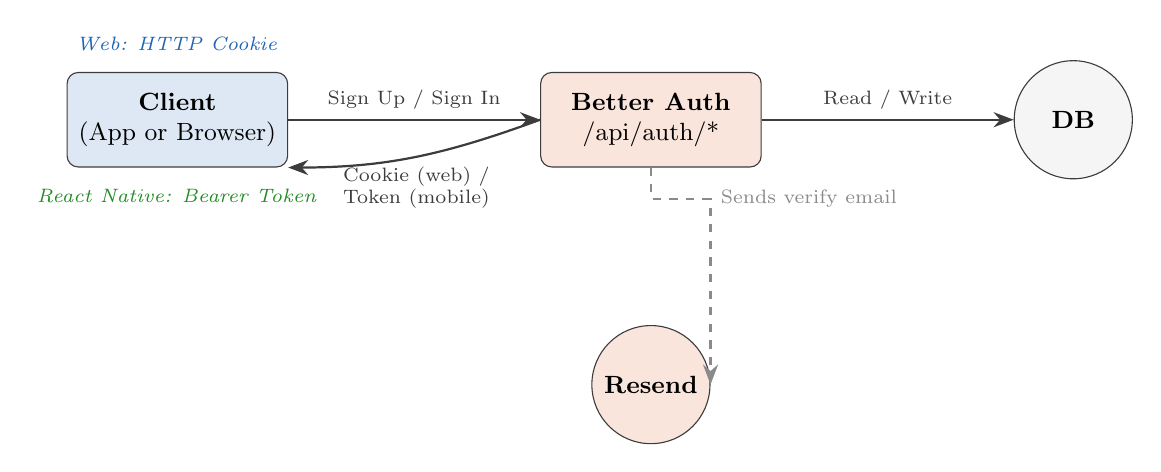
\begin{tikzpicture}[node distance=1.4cm and 2.4cm, every node/.style={font=\small, align=center}]
  \node[rectangle, draw=darkgray, rounded corners=4pt, fill=primaryblue!15, minimum width=2.8cm, minimum height=1.2cm] (client)
        {\textbf{Client}\\(App or Browser)};
  \node[rectangle, draw=darkgray, rounded corners=4pt, fill=accentorange!15, right=3.2cm of client, minimum width=2.8cm, minimum height=1.2cm] (betterauth)
        {\textbf{Better Auth}\\/api/auth/*};
  \node[circle, draw=darkgray, fill=lightgray, minimum size=1.5cm, right=3.2cm of betterauth] (db2)
        {\textbf{DB}};
  \node[circle, draw=darkgray, fill=accentorange!15, below=2cm of betterauth, minimum size=1.5cm] (resend2)
        {\textbf{Resend}};

  \draw[arrow] (client) -- node[above,font=\scriptsize]{Sign Up / Sign In} (betterauth);
  \draw[arrow] (betterauth) -- node[above,font=\scriptsize]{Read / Write} (db2);
  \draw[dasharrow] (betterauth.south) -- ++(0,-0.4) -| node[right,font=\scriptsize]{Sends verify email} (resend2.east);
  \draw[arrow] (betterauth.west) to[out=200,in=0] node[below,font=\scriptsize,align=center]{Cookie (web) /\\Token (mobile)} (client.south east);

  \node[font=\scriptsize, color=successgreen, below=0.15cm of client]
       {\textit{React Native: Bearer Token}};
  \node[font=\scriptsize, color=primaryblue, above=0.15cm of client]
       {\textit{Web: HTTP Cookie}};
\end{tikzpicture}
\end{center}
\newpage
% ═══════════════════════════════════════════════════════════
%  6. TOOLS AND TECHNOLOGIES
% ═══════════════════════════════════════════════════════════
\section{Tools and Technologies Used}

\subsection{Backend Technologies}

\vspace{4pt}
\begin{center}
\renewcommand{\arraystretch}{1.35}
\begin{tabular}{@{} L{3.6cm} L{7.2cm} L{2.6cm} @{}}
\toprule
\rowcolor{tablebg}
\textbf{Technology} & \textbf{Purpose} & \textbf{Version} \\
\midrule
Node.js              & JavaScript runtime for the server             & v20 LTS \\
Express.js           & HTTP framework, routing, middleware            & v4.19 \\
TypeScript           & Static typing for reliability                  & v5.5 \\
Drizzle ORM          & Type-safe SQL query builder                    & v0.36 \\
Better Auth          & Authentication (email, OAuth, sessions)        & v1.2 \\
Zod                  & Request validation schemas                     & v4.0 \\
Neon PostgreSQL      & Serverless PostgreSQL database                 & latest \\
Resend               & Transactional email delivery                   & v3.4 \\
Helmet               & HTTP security headers                          & v8.1 \\
express-rate-limit   & Request rate limiting                          & v8.3 \\
Morgan               & HTTP request logging                           & v1.10 \\
nanoid               & Unique ID generation                           & v5.0 \\
tsx                  & TypeScript execution (dev)                     & v4.15 \\
Docker               & Containerisation for deployment                & latest \\
Fly.io               & Cloud deployment platform                      & --- \\
\bottomrule
\end{tabular}
\end{center}

\subsection{Frontend / Mobile Technologies}

\vspace{4pt}
\begin{center}
\renewcommand{\arraystretch}{1.35}
\begin{tabular}{@{} L{3.6cm} L{9.8cm} @{}}
\toprule
\rowcolor{tablebg}
\textbf{Technology} & \textbf{Purpose} \\
\midrule
React Native             & Cross-platform mobile application (Android + iOS) \\
Expo SDK                 & Managed React Native workflow \\
Expo Router              & File-based navigation \\
NativeWind               & Tailwind CSS for React Native styling \\
TanStack Query           & Server state management and caching \\
Axios                    & HTTP client with Bearer token interceptor \\
expo-secure-store        & Secure token storage on device \\
expo-location            & GPS location capture \\
react-hook-form + Zod    & Form validation on mobile \\
\bottomrule
\end{tabular}
\end{center}

\subsection{Development Tools}

\vspace{4pt}
\begin{center}
\renewcommand{\arraystretch}{1.35}
\begin{tabular}{@{} L{3.6cm} L{9.8cm} @{}}
\toprule
\rowcolor{tablebg}
\textbf{Tool} & \textbf{Purpose} \\
\midrule
Visual Studio Code   & Primary code editor \\
Postman              & API testing and documentation \\
Git + GitHub         & Version control and collaboration \\
drizzle-kit          & Database migration management \\
Docker Desktop       & Local container testing \\
Neon Dashboard       & Database management and SQL editor \\
Fly.io CLI           & Cloud deployment and secret management \\
\bottomrule
\end{tabular}
\end{center}

\newpage
% ═══════════════════════════════════════════════════════════
%  7. SYSTEM REQUIREMENTS
% ═══════════════════════════════════════════════════════════
\section{System Requirements (Hardware \& Software)}

\subsection{Hardware Requirements}

\vspace{4pt}
\begin{center}
\renewcommand{\arraystretch}{1.35}
\begin{tabular}{@{} L{3.6cm} L{5.6cm} L{4cm} @{}}
\toprule
\rowcolor{tablebg}
\textbf{Component} & \textbf{Development} & \textbf{Production (Fly.io)} \\
\midrule
Processor     & Intel Core i5 / AMD Ryzen 5 or better & Shared CPU (1 vCPU) \\
RAM           & 8\,GB minimum, 16\,GB recommended     & 256\,MB minimum \\
Storage       & 20\,GB free disk space                & 3\,GB (Fly.io free tier) \\
Network       & Broadband internet connection          & 160\,GB outbound / month \\
Mobile Device & Android 10+ / iOS 14+ for testing     & --- \\
\bottomrule
\end{tabular}
\end{center}

\subsection{Software Requirements}

\vspace{4pt}
\begin{center}
\renewcommand{\arraystretch}{1.35}
\begin{tabular}{@{} L{3.6cm} L{9.8cm} @{}}
\toprule
\rowcolor{tablebg}
\textbf{Component} & \textbf{Requirement} \\
\midrule
Operating System  & Windows 10/11, macOS 12+, or Ubuntu 22.04 \\
Node.js           & v20 LTS or higher \\
npm               & v10 or higher \\
Docker            & Docker Desktop (Windows/Mac) or Docker Engine (Linux) \\
Git               & v2.40+ \\
PostgreSQL Client & Any (Neon serverless --- no local Postgres needed) \\
IDE               & Visual Studio Code with ESLint and TypeScript extensions \\
Browser           & Google Chrome / Firefox (for API docs at \texttt{/api/docs}) \\
Postman           & v10+ (for API testing) \\
Expo CLI          & For React Native development and testing \\
Android Studio    & For Android emulator (mobile testing) \\
\bottomrule
\end{tabular}
\end{center}

\subsection{API Endpoints Summary}

The backend exposes \textbf{50 REST API endpoints} across 8 resource domains:

\vspace{4pt}
\begin{center}
\renewcommand{\arraystretch}{1.35}
\begin{tabular}{@{} L{3.4cm} C{2cm} L{7.4cm} @{}}
\toprule
\rowcolor{tablebg}
\textbf{Domain} & \textbf{Endpoints} & \textbf{Key Operations} \\
\midrule
Authentication  & 4  & Sign up, sign in, sign out, get session \\
Volunteer       & 7  & Profile, qualifications, team activations \\
Teams           & 7  & Create, join, leave, manage members \\
Panic / SOS     & 2  & Send alert, check status \\
Issues          & 6  & Report, accept, update status, resolve \\
Disasters       & 7  & Declare, update, team activation \\
Campaigns       & 5  & Create, approve, donate, updates \\
Admin           & 12 & Users, volunteers, stats, notifications \\
\midrule
\textbf{Total}  & \textbf{50} & \\
\bottomrule
\end{tabular}
\end{center}

% ═══════════════════════════════════════════════════════════
%  8. EXPECTED OUTCOMES
% ═══════════════════════════════════════════════════════════
\section{Expected Outcomes}

\begin{enumerate}[leftmargin=*, label=\textbf{\arabic*.}, itemsep=4pt]

  \item \textbf{Functional REST API:} A production-deployed, fully documented
        REST API with 50 endpoints, running on Fly.io with Docker containerisation,
        serving both mobile and web clients simultaneously.

  \item \textbf{React Native Mobile Application:} A cross-platform mobile
        application for Android and iOS covering 20 screens across public,
        user, volunteer, and admin roles --- with offline-friendly design
        for low-connectivity disaster zones.

  \item \textbf{Reduced Emergency Response Time:} By connecting citizens
        directly to verified nearby volunteers using GPS-based matching,
        the platform aims to reduce the time between a panic alert being
        sent and a volunteer acknowledging it.

  \item \textbf{Transparent Relief Fund Management:} Verified campaigns
        with real-time progress tracking ensure donors can see exactly
        how much has been raised and by whom --- building public trust
        in the relief process.

  \item \textbf{Volunteer Network for Bihar:} A structured, ranked, and
        verified volunteer database covering all 38 Bihar districts,
        with qualification tracking (first aid, CPR, rescue, medical, etc.)
        that authorities can leverage during any disaster.

  \item \textbf{Scalable Architecture:} The combination of serverless
        PostgreSQL (Neon), containerised deployment (Docker + Fly.io),
        and a stateless REST API means the system can handle traffic
        spikes during actual disaster events without manual scaling.

  \item \textbf{Academic Contribution:} A complete, end-to-end project
        demonstrating the application of full-stack development, database
        design, API security, geolocation algorithms, and cloud deployment
        --- representing the full scope of a BCA curriculum.

\end{enumerate}

% ═══════════════════════════════════════════════════════════
%  9. PROJECT TIMELINE
% ═══════════════════════════════════════════════════════════
\section{Project Timeline}

\begin{center}
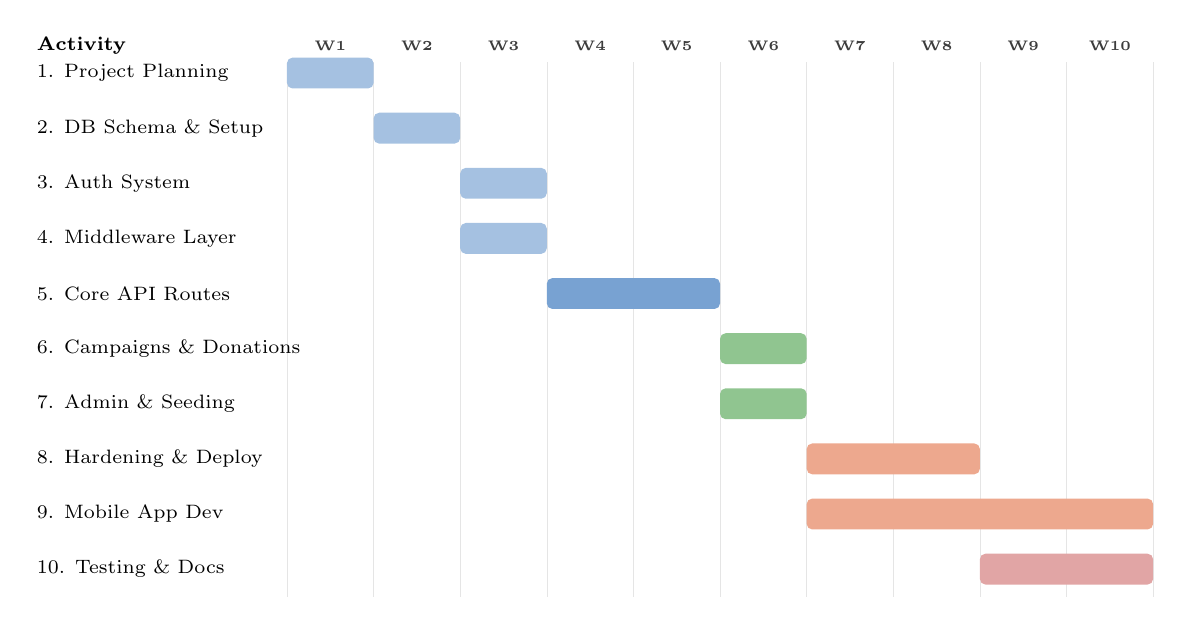
\begin{tikzpicture}[x=1.1cm, y=0.7cm, font=\small]
  % Week labels
  \node[anchor=west, font=\scriptsize\bfseries] at (0,10.5) {Activity};
  \node[font=\tiny\bfseries, color=darkgray] at (3.5,10.5) {W1};
  \node[font=\tiny\bfseries, color=darkgray] at (4.5,10.5) {W2};
  \node[font=\tiny\bfseries, color=darkgray] at (5.5,10.5) {W3};
  \node[font=\tiny\bfseries, color=darkgray] at (6.5,10.5) {W4};
  \node[font=\tiny\bfseries, color=darkgray] at (7.5,10.5) {W5};
  \node[font=\tiny\bfseries, color=darkgray] at (8.5,10.5) {W6};
  \node[font=\tiny\bfseries, color=darkgray] at (9.5,10.5) {W7};
  \node[font=\tiny\bfseries, color=darkgray] at (10.5,10.5) {W8};
  \node[font=\tiny\bfseries, color=darkgray] at (11.5,10.5) {W9};
  \node[font=\tiny\bfseries, color=darkgray] at (12.5,10.5) {W10};
  % Gridlines
  \foreach \wx in {3,4,5,6,7,8,9,10,11,12,13}{
    \draw[gray!20, very thin] (\wx, 0.5) -- (\wx, 10.2);
  }
  % Bars - each row manually
  \node[anchor=west, font=\scriptsize] at (0,10) {1. Project Planning};
  \fill[primaryblue!40, rounded corners=2pt] (3,9.72) rectangle (4,10.28);
  \node[anchor=west, font=\scriptsize] at (0,9) {2. DB Schema \& Setup};
  \fill[primaryblue!40, rounded corners=2pt] (4,8.72) rectangle (5,9.28);
  \node[anchor=west, font=\scriptsize] at (0,8) {3. Auth System};
  \fill[primaryblue!40, rounded corners=2pt] (5,7.72) rectangle (6,8.28);
  \node[anchor=west, font=\scriptsize] at (0,7) {4. Middleware Layer};
  \fill[primaryblue!40, rounded corners=2pt] (5,6.72) rectangle (6,7.28);
  \node[anchor=west, font=\scriptsize] at (0,6) {5. Core API Routes};
  \fill[primaryblue!60, rounded corners=2pt] (6,5.72) rectangle (8,6.28);
  \node[anchor=west, font=\scriptsize] at (0,5) {6. Campaigns \& Donations};
  \fill[successgreen!50, rounded corners=2pt] (8,4.72) rectangle (9,5.28);
  \node[anchor=west, font=\scriptsize] at (0,4) {7. Admin \& Seeding};
  \fill[successgreen!50, rounded corners=2pt] (8,3.72) rectangle (9,4.28);
  \node[anchor=west, font=\scriptsize] at (0,3) {8. Hardening \& Deploy};
  \fill[accentorange!50, rounded corners=2pt] (9,2.72) rectangle (11,3.28);
  \node[anchor=west, font=\scriptsize] at (0,2) {9. Mobile App Dev};
  \fill[accentorange!50, rounded corners=2pt] (9,1.72) rectangle (13,2.28);
  \node[anchor=west, font=\scriptsize] at (0,1) {10. Testing \& Docs};
  \fill[warningred!40, rounded corners=2pt] (11,0.72) rectangle (13,1.28);
\end{tikzpicture}
\end{center}

\begin{center}
\begin{tabularx}{\textwidth}{c >{\bfseries}p{4.5cm} X}
\toprule
\textbf{Phase} & \textbf{Activity} & \textbf{Deliverable} \\
\midrule
1 & Project Planning \& Research & Requirements, schema design \\
2 & Database Schema \& Setup     & 19-table PostgreSQL schema + migrations \\
3 & Auth System                  & Better Auth, email verification, OAuth \\
4 & Middleware Layer             & Auth guards, role checks, Zod validation \\
5 & Core API Routes              & 31 endpoints (volunteer, issues, disasters) \\
6 & Campaigns \& Donations       & Campaign workflow, donation processing \\
7 & Admin Routes \& Seed Data    & 12 admin endpoints, 38 districts seeded \\
8 & Hardening \& Deployment      & Security, rate limiting, Docker, Fly.io \\
9 & Mobile App Development       & React Native 20-screen application \\
10& Testing \& Documentation     & Postman collection, API docs, final report \\
\bottomrule
\end{tabularx}
\end{center}

% ═══════════════════════════════════════════════════════════
%  10. REFERENCES
% ═══════════════════════════════════════════════════════════
\section{References}

\begin{enumerate}[leftmargin=*, label={[\arabic*]}, itemsep=4pt]

  \item National Disaster Management Authority (NDMA), Government of India.
        \textit{Bihar Flood Management Report}.
        Available at: \url{https://ndma.gov.in}

  \item Better Auth Documentation.
        \textit{Authentication for modern web applications}.
        Available at: \url{https://better-auth.com/docs}

  \item Drizzle ORM Documentation.
        \textit{TypeScript ORM for SQL databases}.
        Available at: \url{https://orm.drizzle.team}

  \item Neon Database.
        \textit{Serverless PostgreSQL}.
        Available at: \url{https://neon.tech/docs}

  \item Express.js Documentation.
        \textit{Fast, unopinionated, minimalist web framework for Node.js}.
        Available at: \url{https://expressjs.com}

  \item React Native Documentation.
        \textit{Learn once, write anywhere}.
        Available at: \url{https://reactnative.dev/docs}

  \item Expo Documentation.
        \textit{An open-source platform for making universal native apps}.
        Available at: \url{https://docs.expo.dev}

  \item Fly.io Documentation.
        \textit{Deploy app servers close to your users}.
        Available at: \url{https://fly.io/docs}

  \item Pressman, R.S. (2014).
        \textit{Software Engineering: A Practitioner's Approach}, 8th ed.
        McGraw-Hill Education.

  \item Silberschatz, A., Korth, H.F., \& Sudarshan, S. (2019).
        \textit{Database System Concepts}, 7th ed.
        McGraw-Hill Education.

  \item Resend Email API Documentation.
        Available at: \url{https://resend.com/docs}

  \item OWASP Foundation.
        \textit{OWASP Top Ten Security Risks}.
        Available at: \url{https://owasp.org/www-project-top-ten}

\end{enumerate}


\vspace{2cm}
\noindent\textcolor{darkgray!40}{\rule{\textwidth}{0.4pt}}

\vspace{1.2cm}
\begin{tabular}{@{} L{7cm} L{7cm} @{}}
\textbf{Student 1 Signature} & \textbf{Student 2 Signature} \\[0.4cm]
Name:\ \ Shubham Kumar Mishra & Name:\ \ Atul Sharma \\
Roll No:\ \ 23                & Roll No:\ \ 10 \\
BCA Sem V, Batch 2023--26    & BCA Sem V, Batch 2023--26 \\[1.8cm]
\underline{\hspace{5.5cm}}   & \underline{\hspace{5.5cm}} \\[1.2cm]
\end{tabular}

\begin{tabular}{@{} L{7cm} L{7cm} @{}}
\textbf{Project Guide Signature} & \textbf{HOD Signature} \\[0.4cm]
Name:\ \ \underline{\hspace{4.5cm}} & Name:\ \ \underline{\hspace{4.5cm}} \\
Designation:\ \ \underline{\hspace{3.8cm}} & \\[1.8cm]
\underline{\hspace{5.5cm}} & \underline{\hspace{5.5cm}} \\
\end{tabular}

\end{document}